\section{Testing Simulations}
\label{appendix::gabby}

As an initial exploration into the consequences of continued
\ac{kasat} testing, the question was posed: ``What would it look like
if some number of tests were to happen each year at random times?''
In answer to that question, the
\href{https://github.com/harrison-caudill/gabby}{Gabby software
  package} was used to ``simulate'' two scenarios.  The extent of the
``simulation'' was effectively to combine, for convenience, the output
of two prior publications: the
\href{https://www.youtube.com/watch?v=InBMUkH1i9Q}{Mission Shakti
  Gabbard Animation} and the
\href{https://www.youtube.com/watch?v=U8Y8MNK-L3I}{Nudol Gabbard
  Animation}.

Figure \ref{figure::gabby::doomsday::mix} shows approximately what the
total debris count and distribution might look like if three tests per
year were to occur randomly.  This figure shows the results of a mix
of $\frac{1}{3}$ Nudol-style events and $\frac{2}{3}$ Shakti-style
events.  As can be seen, the total debris count is quite large,
peaking at around 9,000 pieces of trackable debris.

Figure \ref{figure::gabby::doomsday::shakti} shows a similar scenario,
only restricting tests to those similar to Mission Shakti.  With total
debris topping out close to 1,250 pieces, it becomes immediately
apparent that the conditions of testing matter tremendously in the
overall debris environment.

As further illustration of the consequences of the test conditions,
figure \ref{figure::gabby::doomsday::doom} shows the results of a mix
of $\frac{1}{3}$ Fengyun-style events and $\frac{2}{3}$ Shakti-style
events.  Even the comparatively low orbital altitude of the recent
Nudol ``test'' produces what might be considered an unacceptable
debris environment, and the conditions of China's destruction of
Fengyun-1C are far worse, with the total debris count peaking over
40,000.

\begin{figure}[ht!]
  % ./bin/plot -c ~/dev/nukes/gabby.cfg -n 7 -T doom -t mix
  \begin{center}
    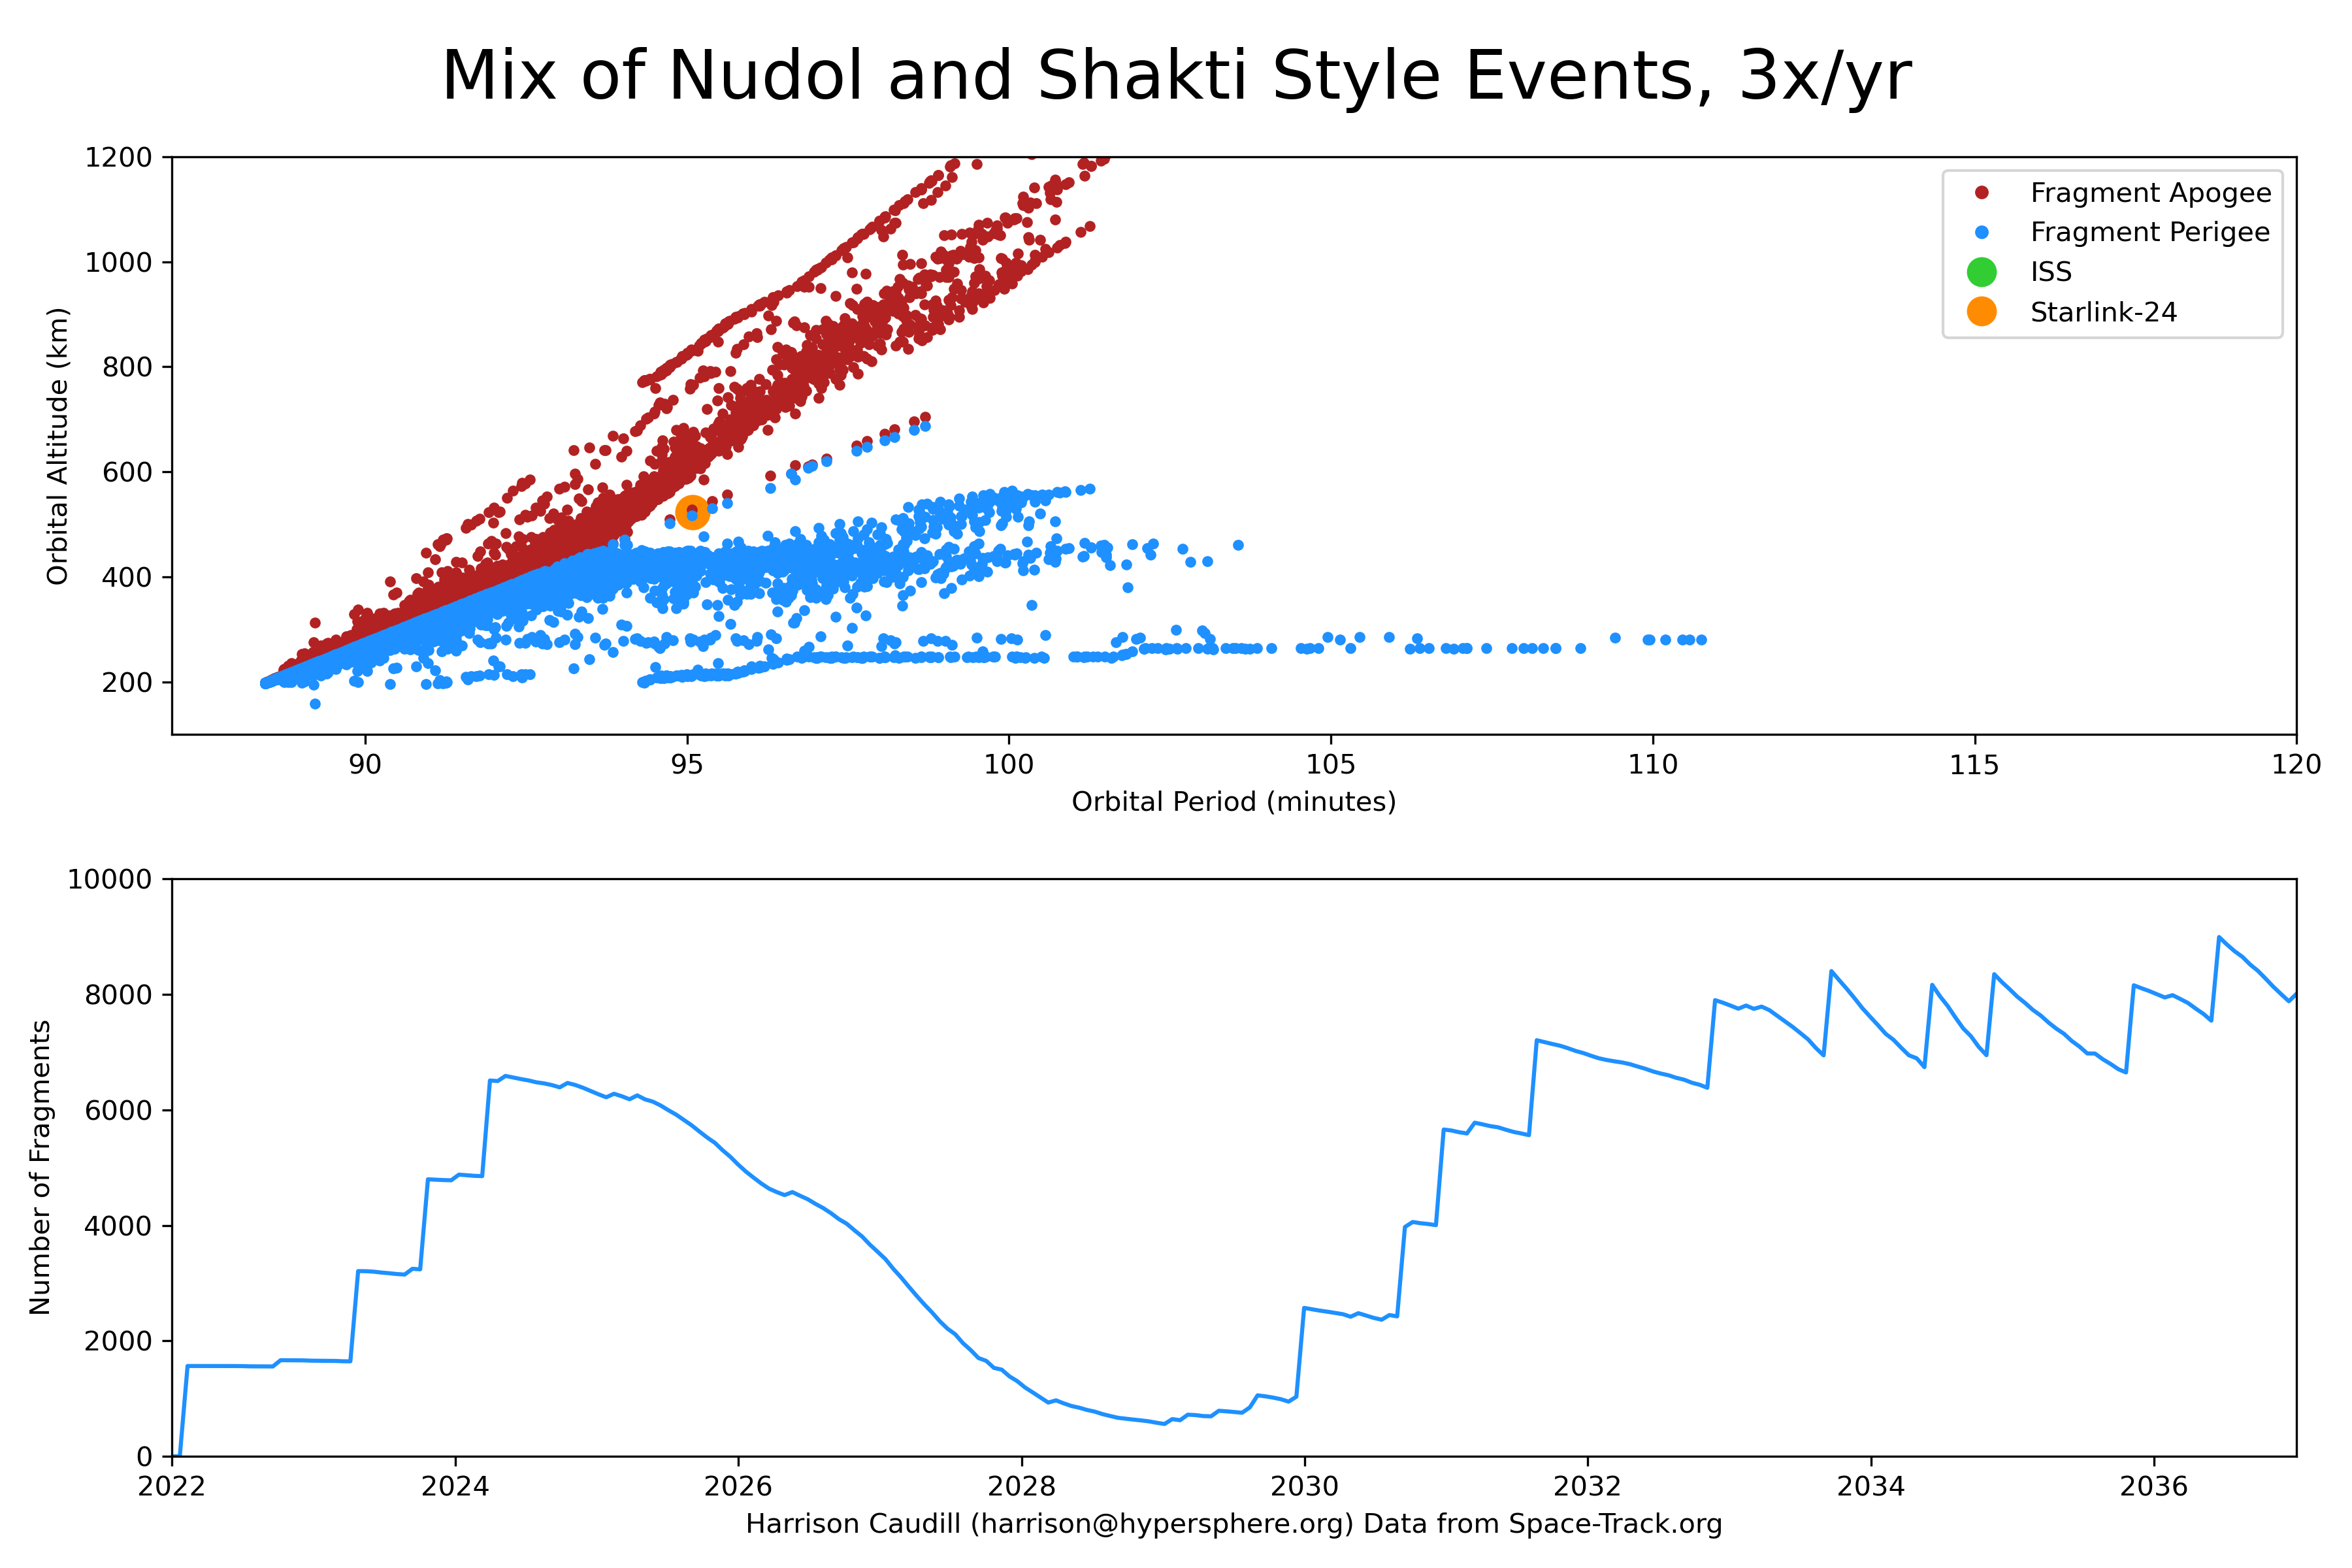
\includegraphics[width=4in]{mix.png}
  \end{center}
  \caption{Simulation of three \ac{asat} tests per year at random
    intervals.  $\frac{1}{3}$ Nudol-style events and $\frac{2}{3}$
    Shakti-style events.}
  \label{figure::gabby::doomsday::mix}
\end{figure}

\begin{figure}[ht!]
  % ./bin/plot -c ~/dev/nukes/gabby.cfg -n 7 -T doom -t shakti
  \begin{center}
    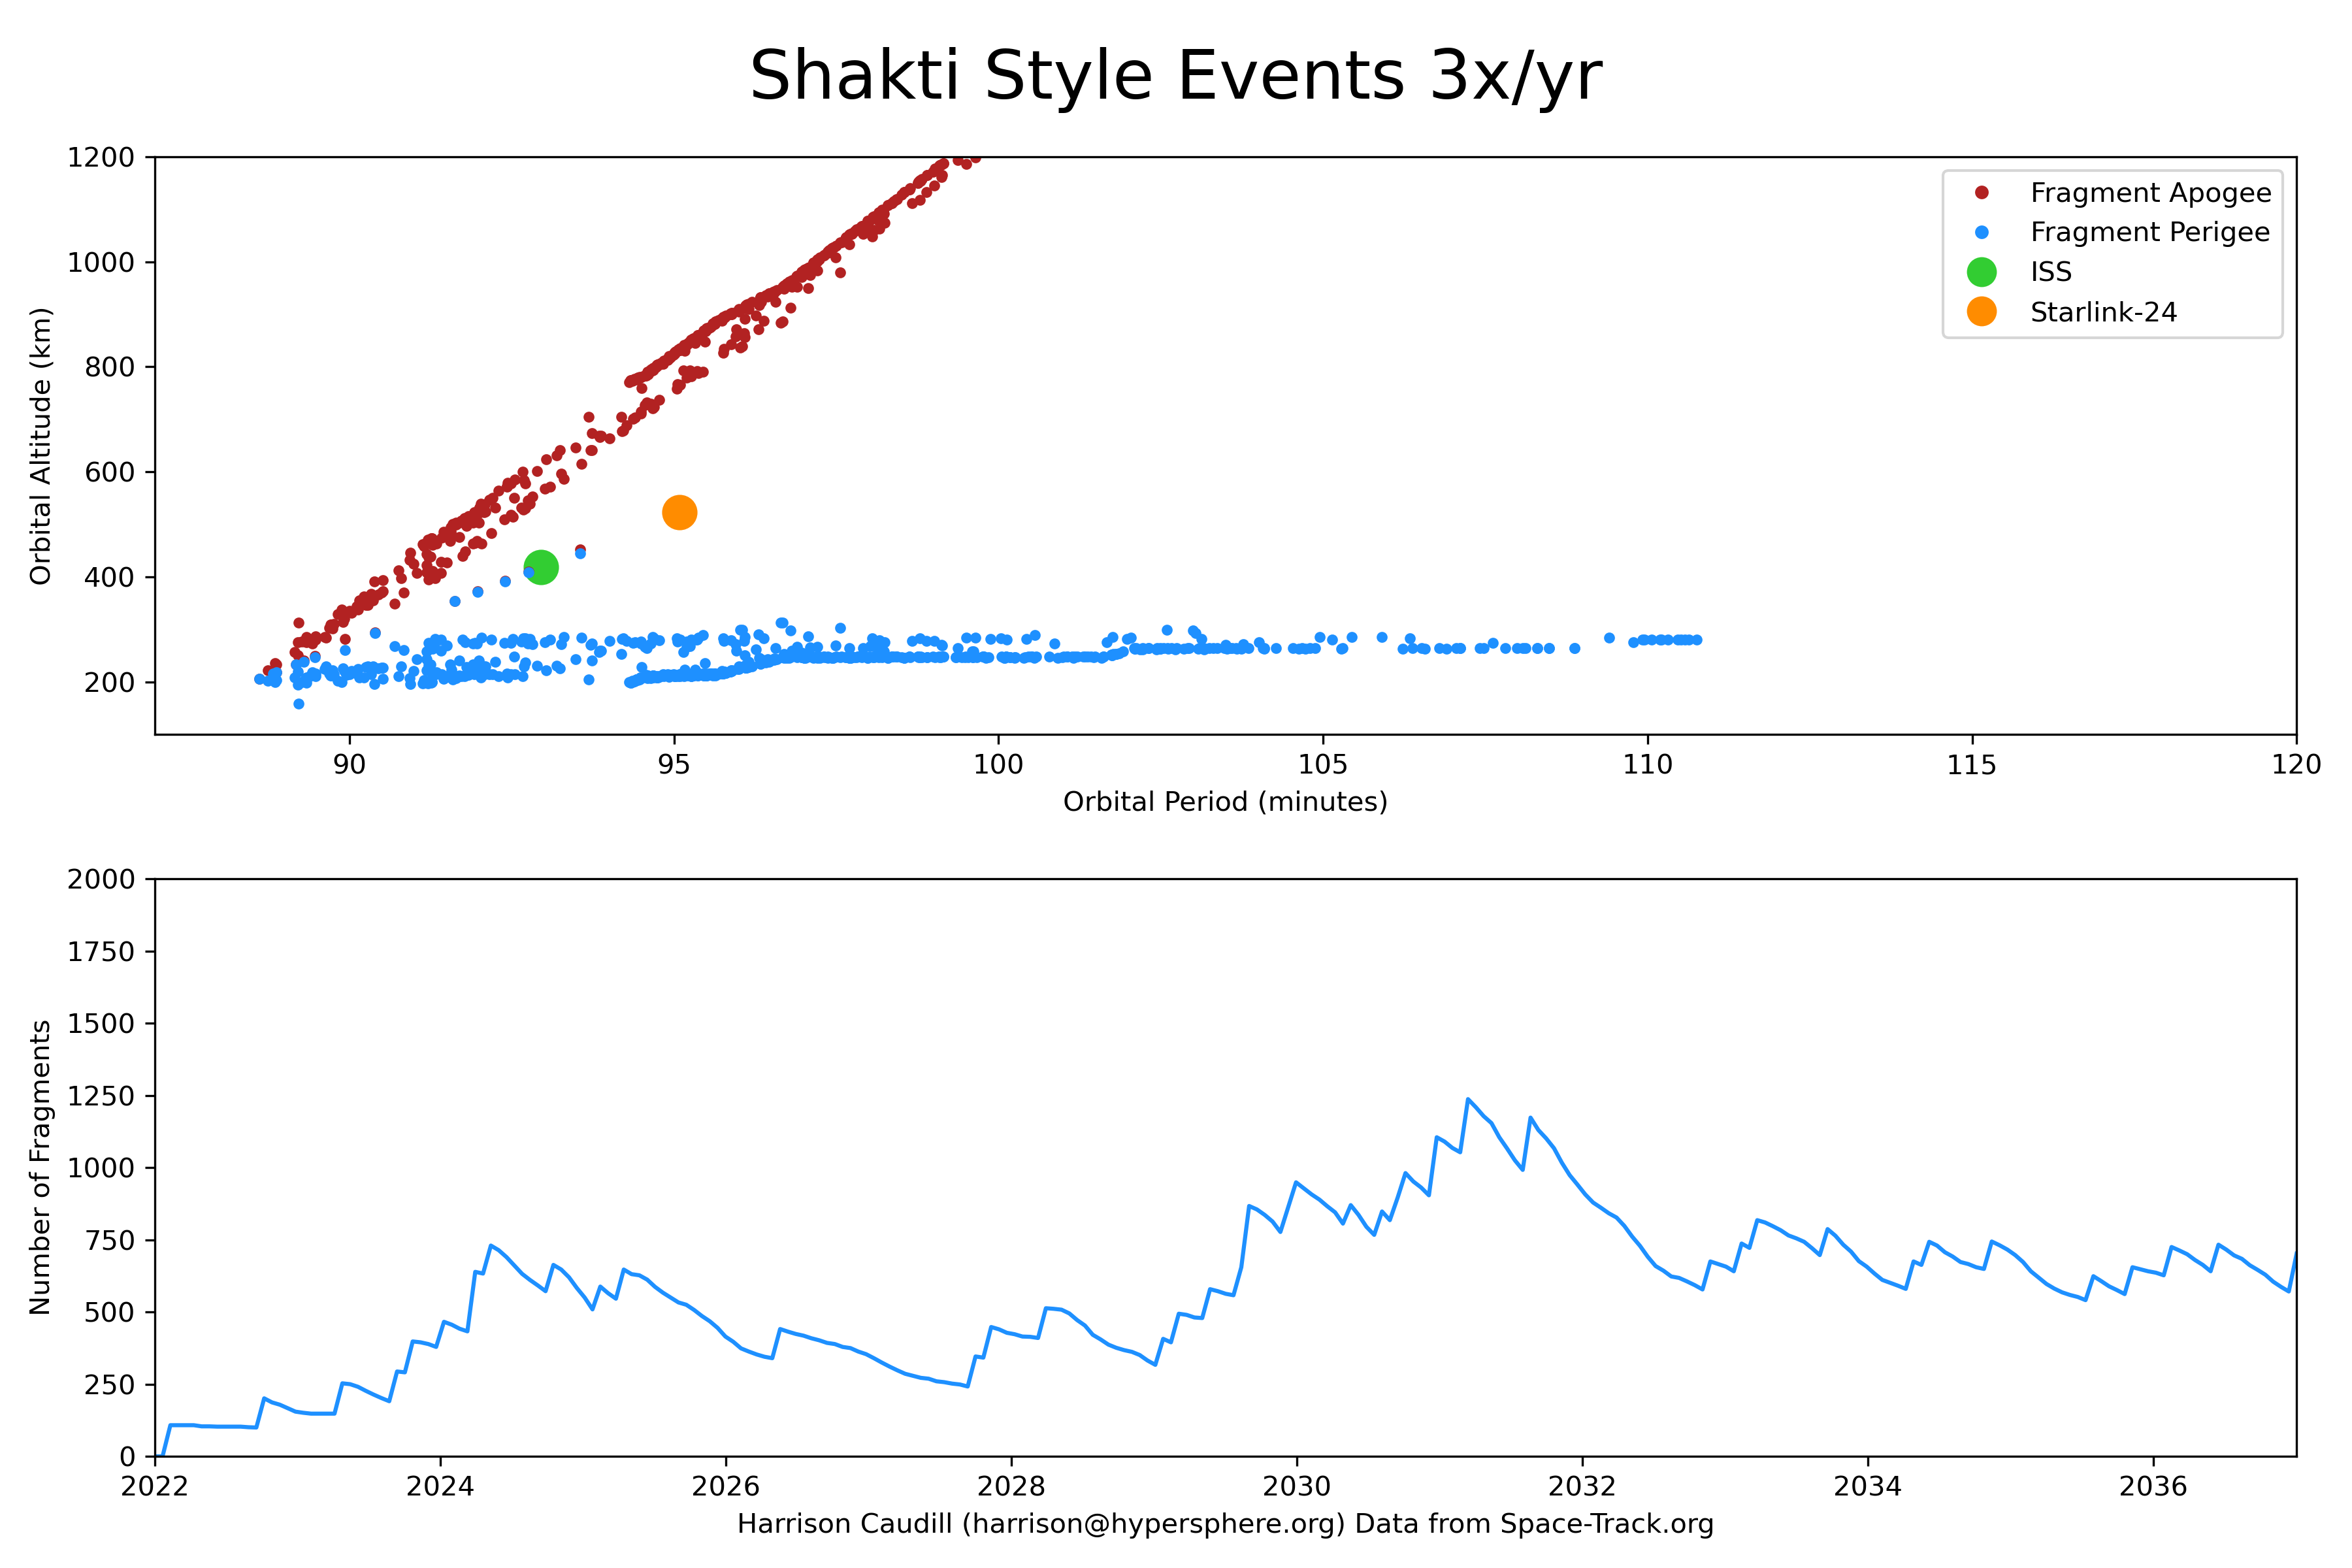
\includegraphics[width=4in]{shakti.png}
  \end{center}
  \caption{Simulation of three Shakti-style \ac{asat} tests per year
    at random intervals.}
  \label{figure::gabby::doomsday::shakti}
\end{figure}

\begin{figure}[ht!]
  % ./bin/plot -c ~/dev/nukes/gabby.cfg -n 7 -T doom -t doom
  \begin{center}
    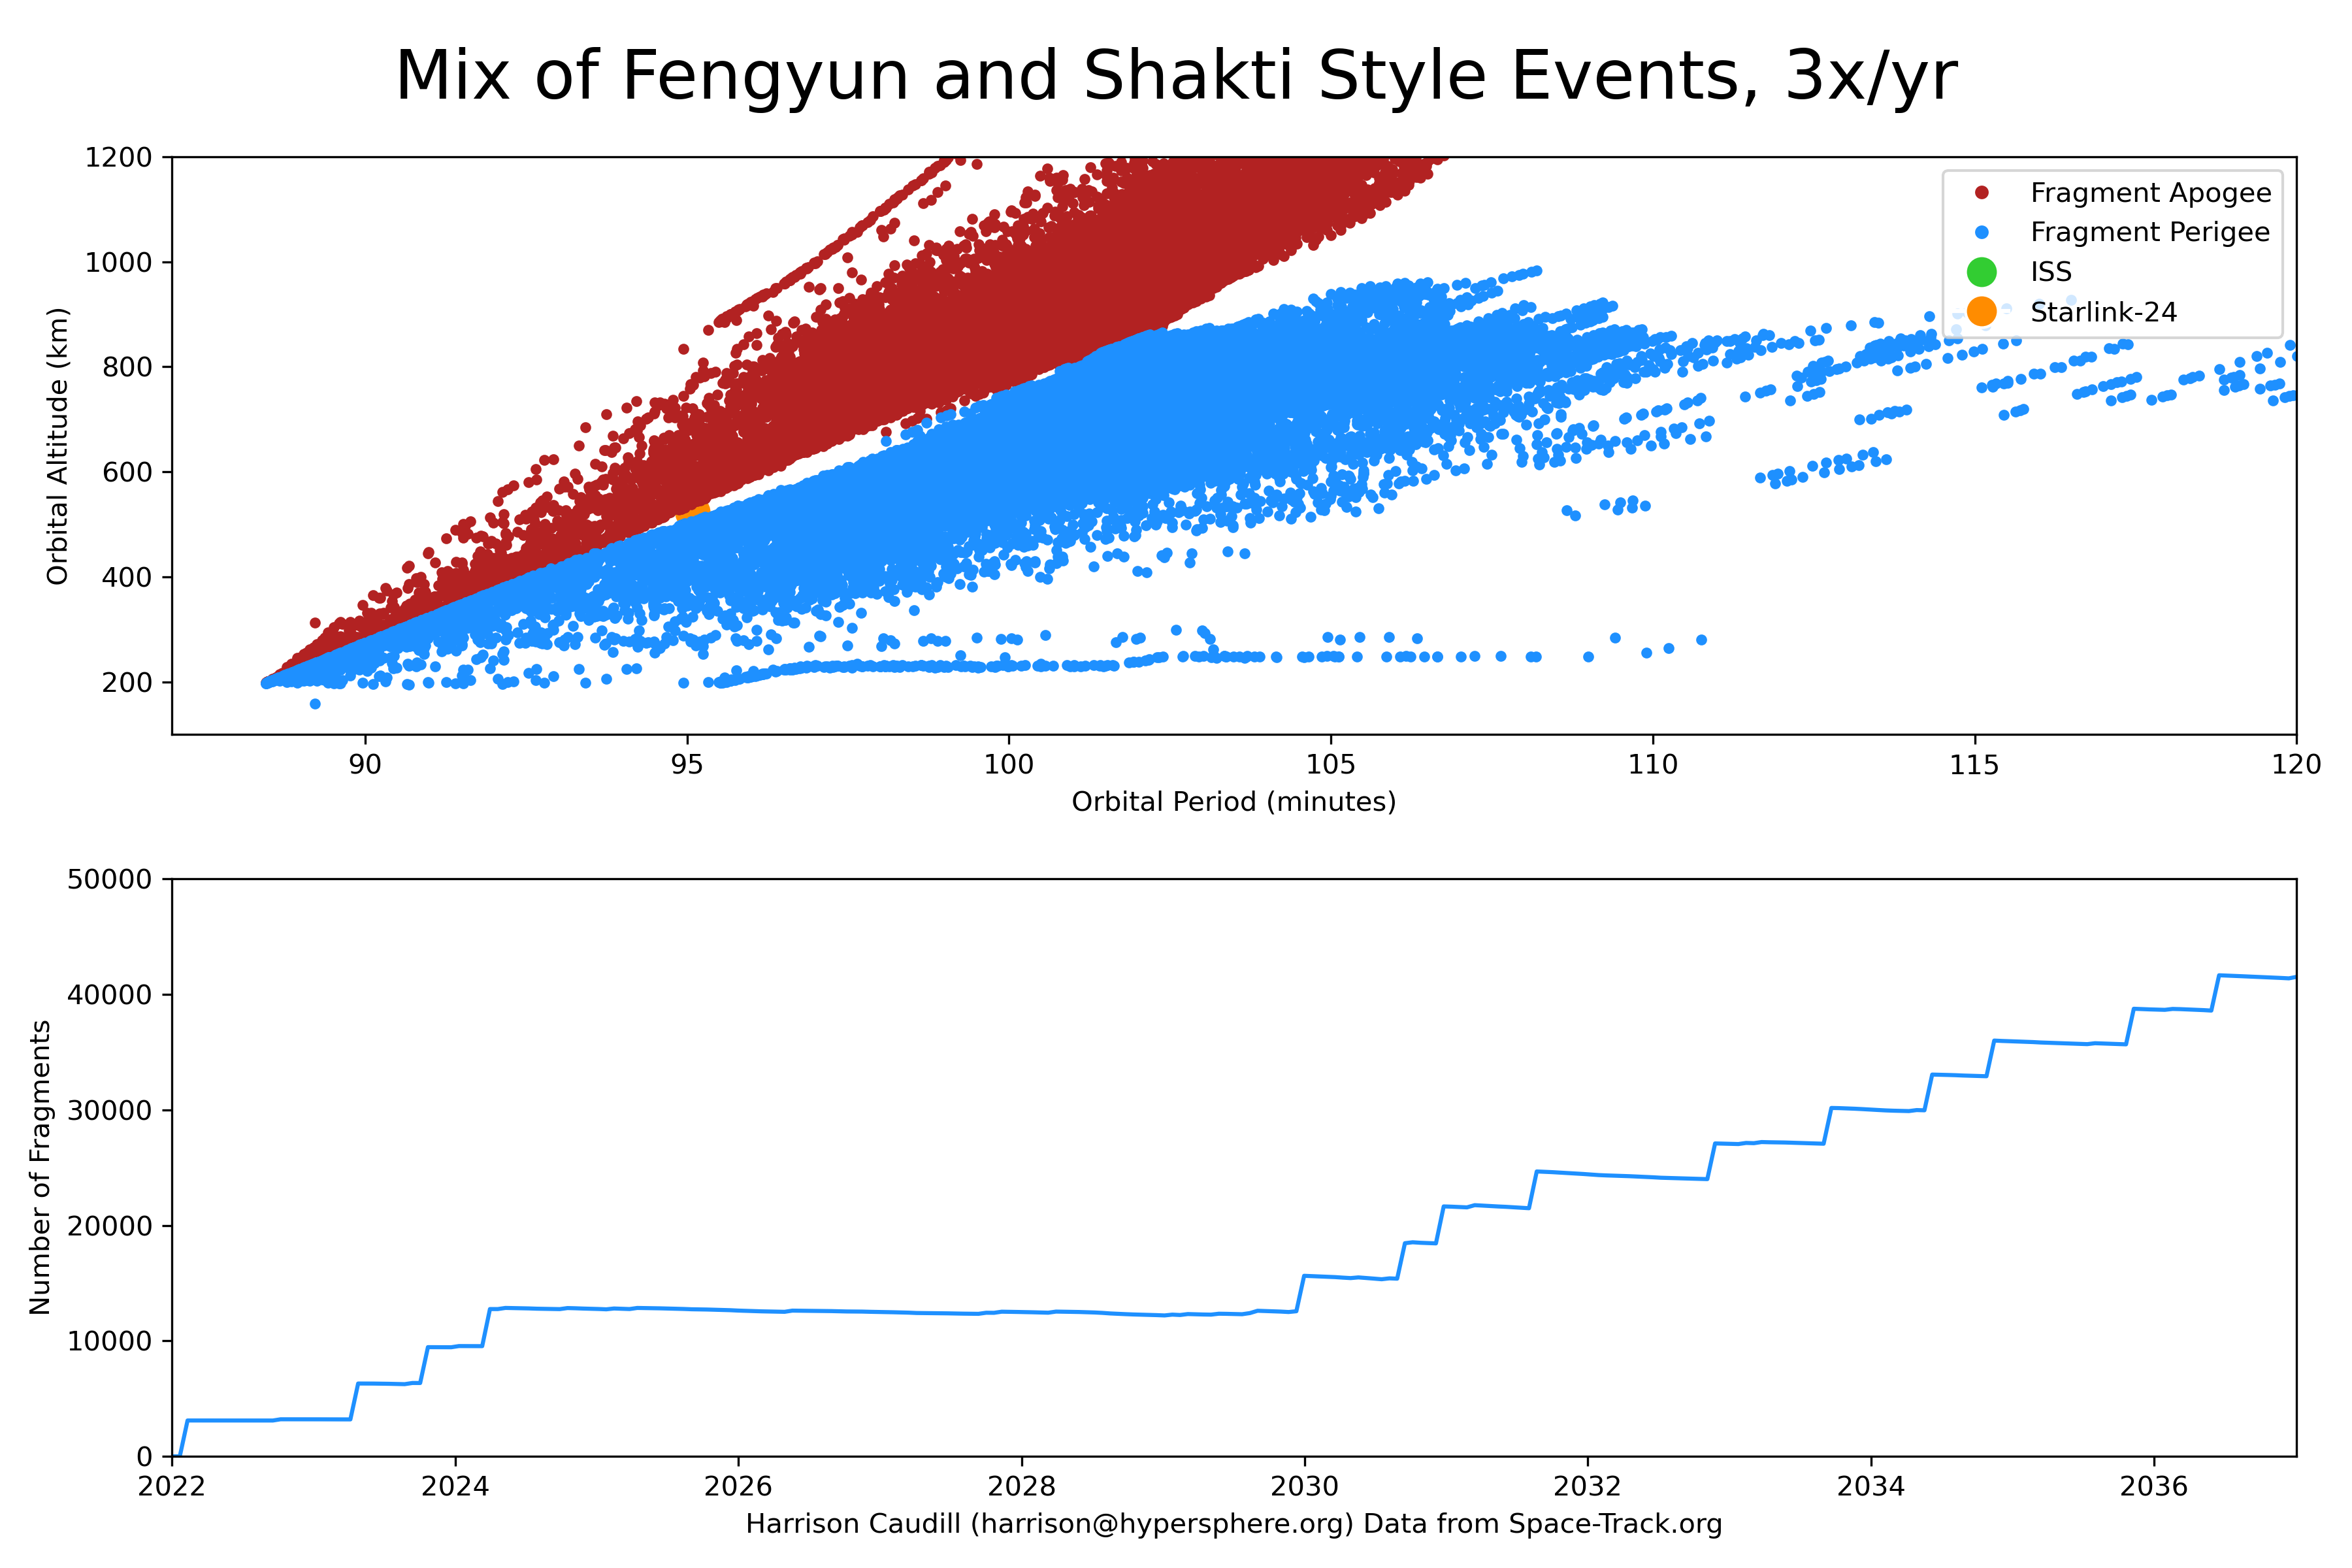
\includegraphics[width=4in]{doom.png}
  \end{center}
  \caption{Simulation of three \ac{asat} tests per year at random
    intervals.  $\frac{1}{3}$ Fengyun-style events and $\frac{2}{3}$
    Shakti-style events.}
  \label{figure::gabby::doomsday::doom}
\end{figure}
